\documentclass[12pt,a4paper]{article}
\special{papersize=210mm,297mm}

%\usepackage[utf8]{inputenc}
\usepackage[english]{babel}
\bibliographystyle{unsrt}

\title{Exercise 10}
\author{Stefan Lenz\\11810302}


%---------------------------------------------------------------------------
%Packages
%---------------------------------------------------------------------------
\usepackage[parfill]{parskip} 

\usepackage[parfill]{parskip} 
\usepackage[pdftex]{graphicx}
\DeclareGraphicsExtensions{.pdf,.png,.jpg}
\usepackage{xcolor}
\usepackage{listings}

\definecolor{mGreen}{rgb}{0,0.6,0}
\definecolor{mGray}{rgb}{0.5,0.5,0.5}
\definecolor{mPurple}{rgb}{0.58,0,0.82}
\definecolor{backgroundColour}{rgb}{0.95,0.95,0.92}

\lstdefinestyle{CStyle}{
    backgroundcolor=\color{backgroundColour},   
    commentstyle=\color{mGreen},
    keywordstyle=\color{magenta},
    numberstyle=\tiny\color{mGray},
    stringstyle=\color{mPurple},
    basicstyle=\footnotesize,
    breakatwhitespace=false,         
    breaklines=true,                 
    captionpos=b,                    
    keepspaces=true,                 
    numbers=left,                    
    numbersep=5pt,                  
    showspaces=false,                
    showstringspaces=false,
    showtabs=false,                  
    tabsize=2,
    language=C
}
\lstset{style=CStyle}
%Kopf und Fußzeilebearbeiten
\usepackage{fancyhdr}
\pagestyle{fancy}
\headheight 10mm
\chead{Stefan Lenz 11810302}
\lhead{WS23}
\rhead{Exercise 10}
%pic in paragraph bilder in Absätzen winbinden
\usepackage{picinpar}
%matheshit
\usepackage{amsmath}
\usepackage{amsfonts}
%Eurosymbol verwendedn
\usepackage{mathtools}
\DeclarePairedDelimiter{\ceil}{\lceil}{\rceil}
\usepackage{eurosym}
%verschiedene textsymbole (copyrightzeichen, ...)
\usepackage{textcomp}
\usepackage{threeparttable} % for footnotes in tables!
\interfootnotelinepenalty=10000 % for longer footnotes on same page
%Improves the interface for defining floating objects such as figures and tables
\usepackage{float}
%zum importieren von grafiken etc.
\usepackage{import}


\setcounter{topnumber}{2}%max 2 top Floats auf Textseiten
\setcounter{bottomnumber}{2}%
\setcounter{totalnumber}{5}% nur max 4 Floats je Seite?
\setcounter{dbltopnumber}{3}%
\renewcommand\topfraction{0.5}%	wieviel Hoehe maximal fuer Floats erlaubt ist
\renewcommand\dbltopfraction{0.5}%	wieviel Hoehe maximal fuer Floats erlaubt ist
\renewcommand\bottomfraction{0.5}% sonst keine grossen Bilder unten [b] platzieren!
\renewcommand\textfraction{0.1}%	Mindestplatz fuer Text wenn Floats auf der Seite

\usepackage[verbose]{placeins} % Zitatstyle
\renewcommand{\arraystretch}{1.5} %tabellen reihenabstand vergrößern
\usepackage[small,bf]{caption}
\usepackage[
labelfont=sf,
hypcap=false,
format=hang,
margin=1cm,
]{caption}

\usepackage{wrapfig}
\usepackage{subfig}
\usepackage{color}
\usepackage[colorlinks = true,
            linkcolor = black,
            urlcolor  = blue,
            citecolor = black,
            anchorcolor = black]{hyperref}

% By default, URLs are printed using mono-spaced fonts. 
% If you don't like it and you want them to be printed 
% with the same style of the rest of the text, you can use this:
%\urlstyle{same}
\usepackage[footnote]{acronym}
\usepackage{hyperref}
\date{}

\begin{document}
\begin{center}
  \section*{Exercise 10}
\end{center}
\subsection*{Random Number List (CPU)}
In this task we should compute the random numbers on the CPU and copy an array to the GPU which then the threads can draw the needed random  numbers from. This was achieved, by computing the maximum number of contacts inside the \lstinline|contacts_per_day| array. With this information an array was created \lstinline|cuda_rand_values_threads| which then contains the maximum possible amount of random numbers that could be needed for one day. Each thread indexes the array via its thread ID multiplyed by the number of \lstinline|max_rand_values_per_thread|, and then adds according for which contact a random number is currently requested. Due to memoryy efficiency it is not practical to copmpute one large array containing all the random numbers for all days of the simulation. The reason behind this, is that most of these numbers are never needed due to the pushback that is implemented.
\subsection*{Random Number Generation on GPU}
In this task we should create our own random number generator on the GPU which is then used to compute the needed random numbers. To achieve this three additional cuda funciton were created:
\begin{itemize}
  \item \textbf{cuda\_taus: } This function performs one Tausworthe step on the state reference and updates the state.
  \item \textbf{cuda\_LCG: } This function performs a linear congruential generator step on the state reference and updates this state.
  \item \textbf{cuda\_gen\_rand\_num: } This function combines one Tausworthe step with one LCG step to generate better random numbers. Then the result is scaled and returned.
\end{itemize}\
The states used are arrays where each thread has its own state for the Tausworthe and LCG steps. These arrays are initialized with random numbers on the CPU und then updated in ech step of the random number generation process. In my implementation one Tausworthe and one LCG steps are combined, but with the given functions this could easily be expanded to use multiple steps. For this simulation after verifying the desired properties of the random numbers generated it suffices to only use these two steps and cut down on computation cost. 
\subsubsection*{Quality of the Random Numbers}
To verify the quality of the generated random numbers an extra program was created, using the same method to compute random numbers on the GPU and afterwards analyzed. The mean was checked and the distribution of the numbers in $0.1$ intervals between zero and one, with the following results.
\begin{lstlisting}
CHECKING STATISICAL QUALITY

Numbers generated: 10000000, in the interval betweene 0 and 1
checking number of values in the given intervals:

Bin 0 (Range 0 to 0.1): 1000288 10.00%
Bin 1 (Range 0.10 to 0.20): 1000191 10.00%
Bin 2 (Range 0.20 to 0.30): 999293 9.99%
Bin 3 (Range 0.30 to 0.40): 1002224 10.02%
Bin 4 (Range 0.40 to 0.50): 997971 9.98%
Bin 5 (Range 0.50 to 0.60): 998875 9.99%
Bin 6 (Range 0.60 to 0.70): 999221 9.99%
Bin 7 (Range 0.70 to 0.80): 1000107 10.00%
Bin 8 (Range 0.80 to 0.90): 1001703 10.02%
Bin 9 (Range 0.90 to 1.00): 1000127 10.00%

Mean: 0.500015
\end{lstlisting}

\subsection*{Port from CPU to GPU}
To port the simualtion from the CPU to the GPU most of the parts in the simulation function were realized with cuda kernels. The specific implementation differs slightly depending on if the random numbers are generated on the CPU or GPU. The general approach is, that first all the necessary arrays are allcoated on the CPU and GPU. After that a cuda kernel is used to generate the initial data array. Then the main loop over the simulation days starts. In this loop a kernel is used to compute the daily number of fake news believers, which then reports the result back to the CPU. The checking if pushback is true, as well as computing th ecorresponding transmissiona and recovery probabilities on the CPU (for these calculation it makes no sense to do this on the GPU because it is only once computed for the day). After that the generated values are used in the final cuda kernel where the fakenews are passed on according to the reference  implementation. Duriung the loop over the days all the data remains on the GPU only the believer count of the current day is reported back to the CPU.
\subsection*{Performance Model}
To assess the performance of the Implementations first the different execution times for the GPU implementation of the usage of the random number list from the CPU compared to the direct computation on the GPU. In \autoref*{fig:population} it can be seen, that the computation directly on the GPU has huge advantage in terms of performance compared to the usage of a precomputed list.
\begin{figure}[H]
    \centering
    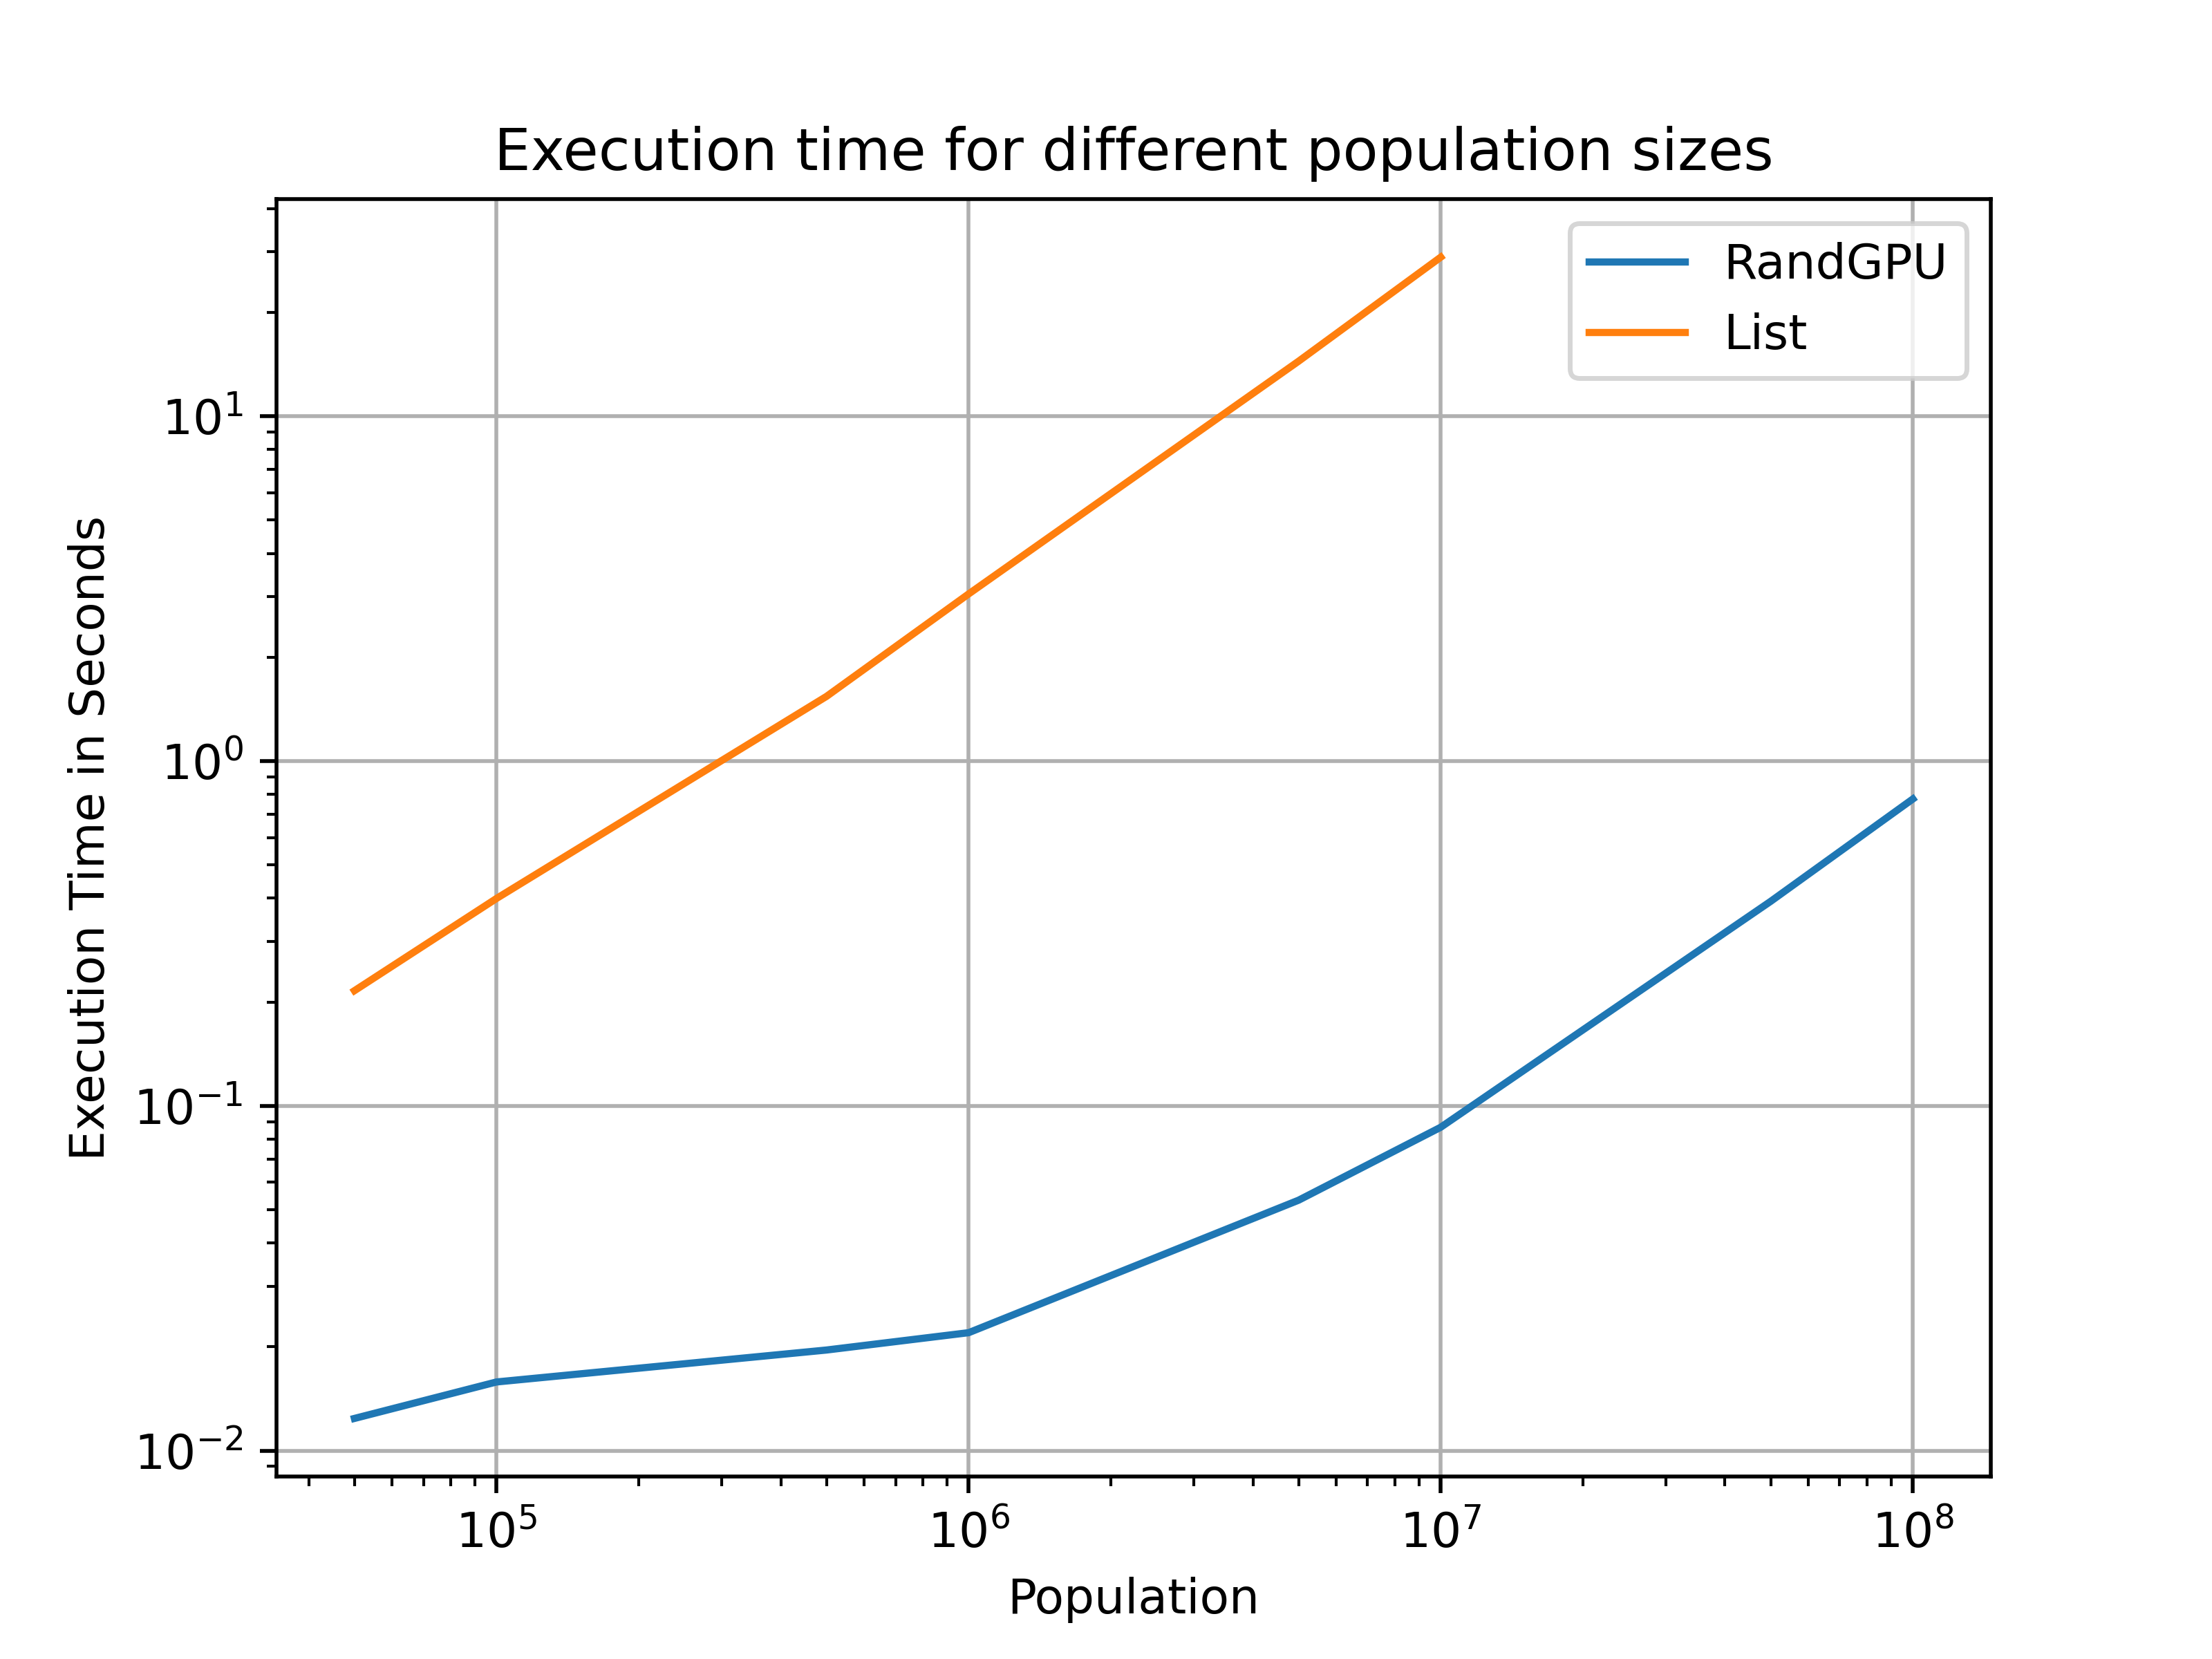
\includegraphics[width=12cm]{../Population.png}
    \caption{Execution times with pushback for different ppopulation sizes.}
    \label{fig:population}
\end{figure}
What is important to note here is, that due to the pushback the variation of the days that are simulated, does not really make a difference due to the fact that the pushback threshold will be reached always at a similar point (provided, that all the other parameters stay the same) which then kills the 'epidemic' at similar points in time. To visualize this the following figure shows the execution times for different population sizes for the program that computes the random numbers on the GPU. The only difference being that pushsback is once disabled and once enabled.
\begin{figure}[H]
    \centering
    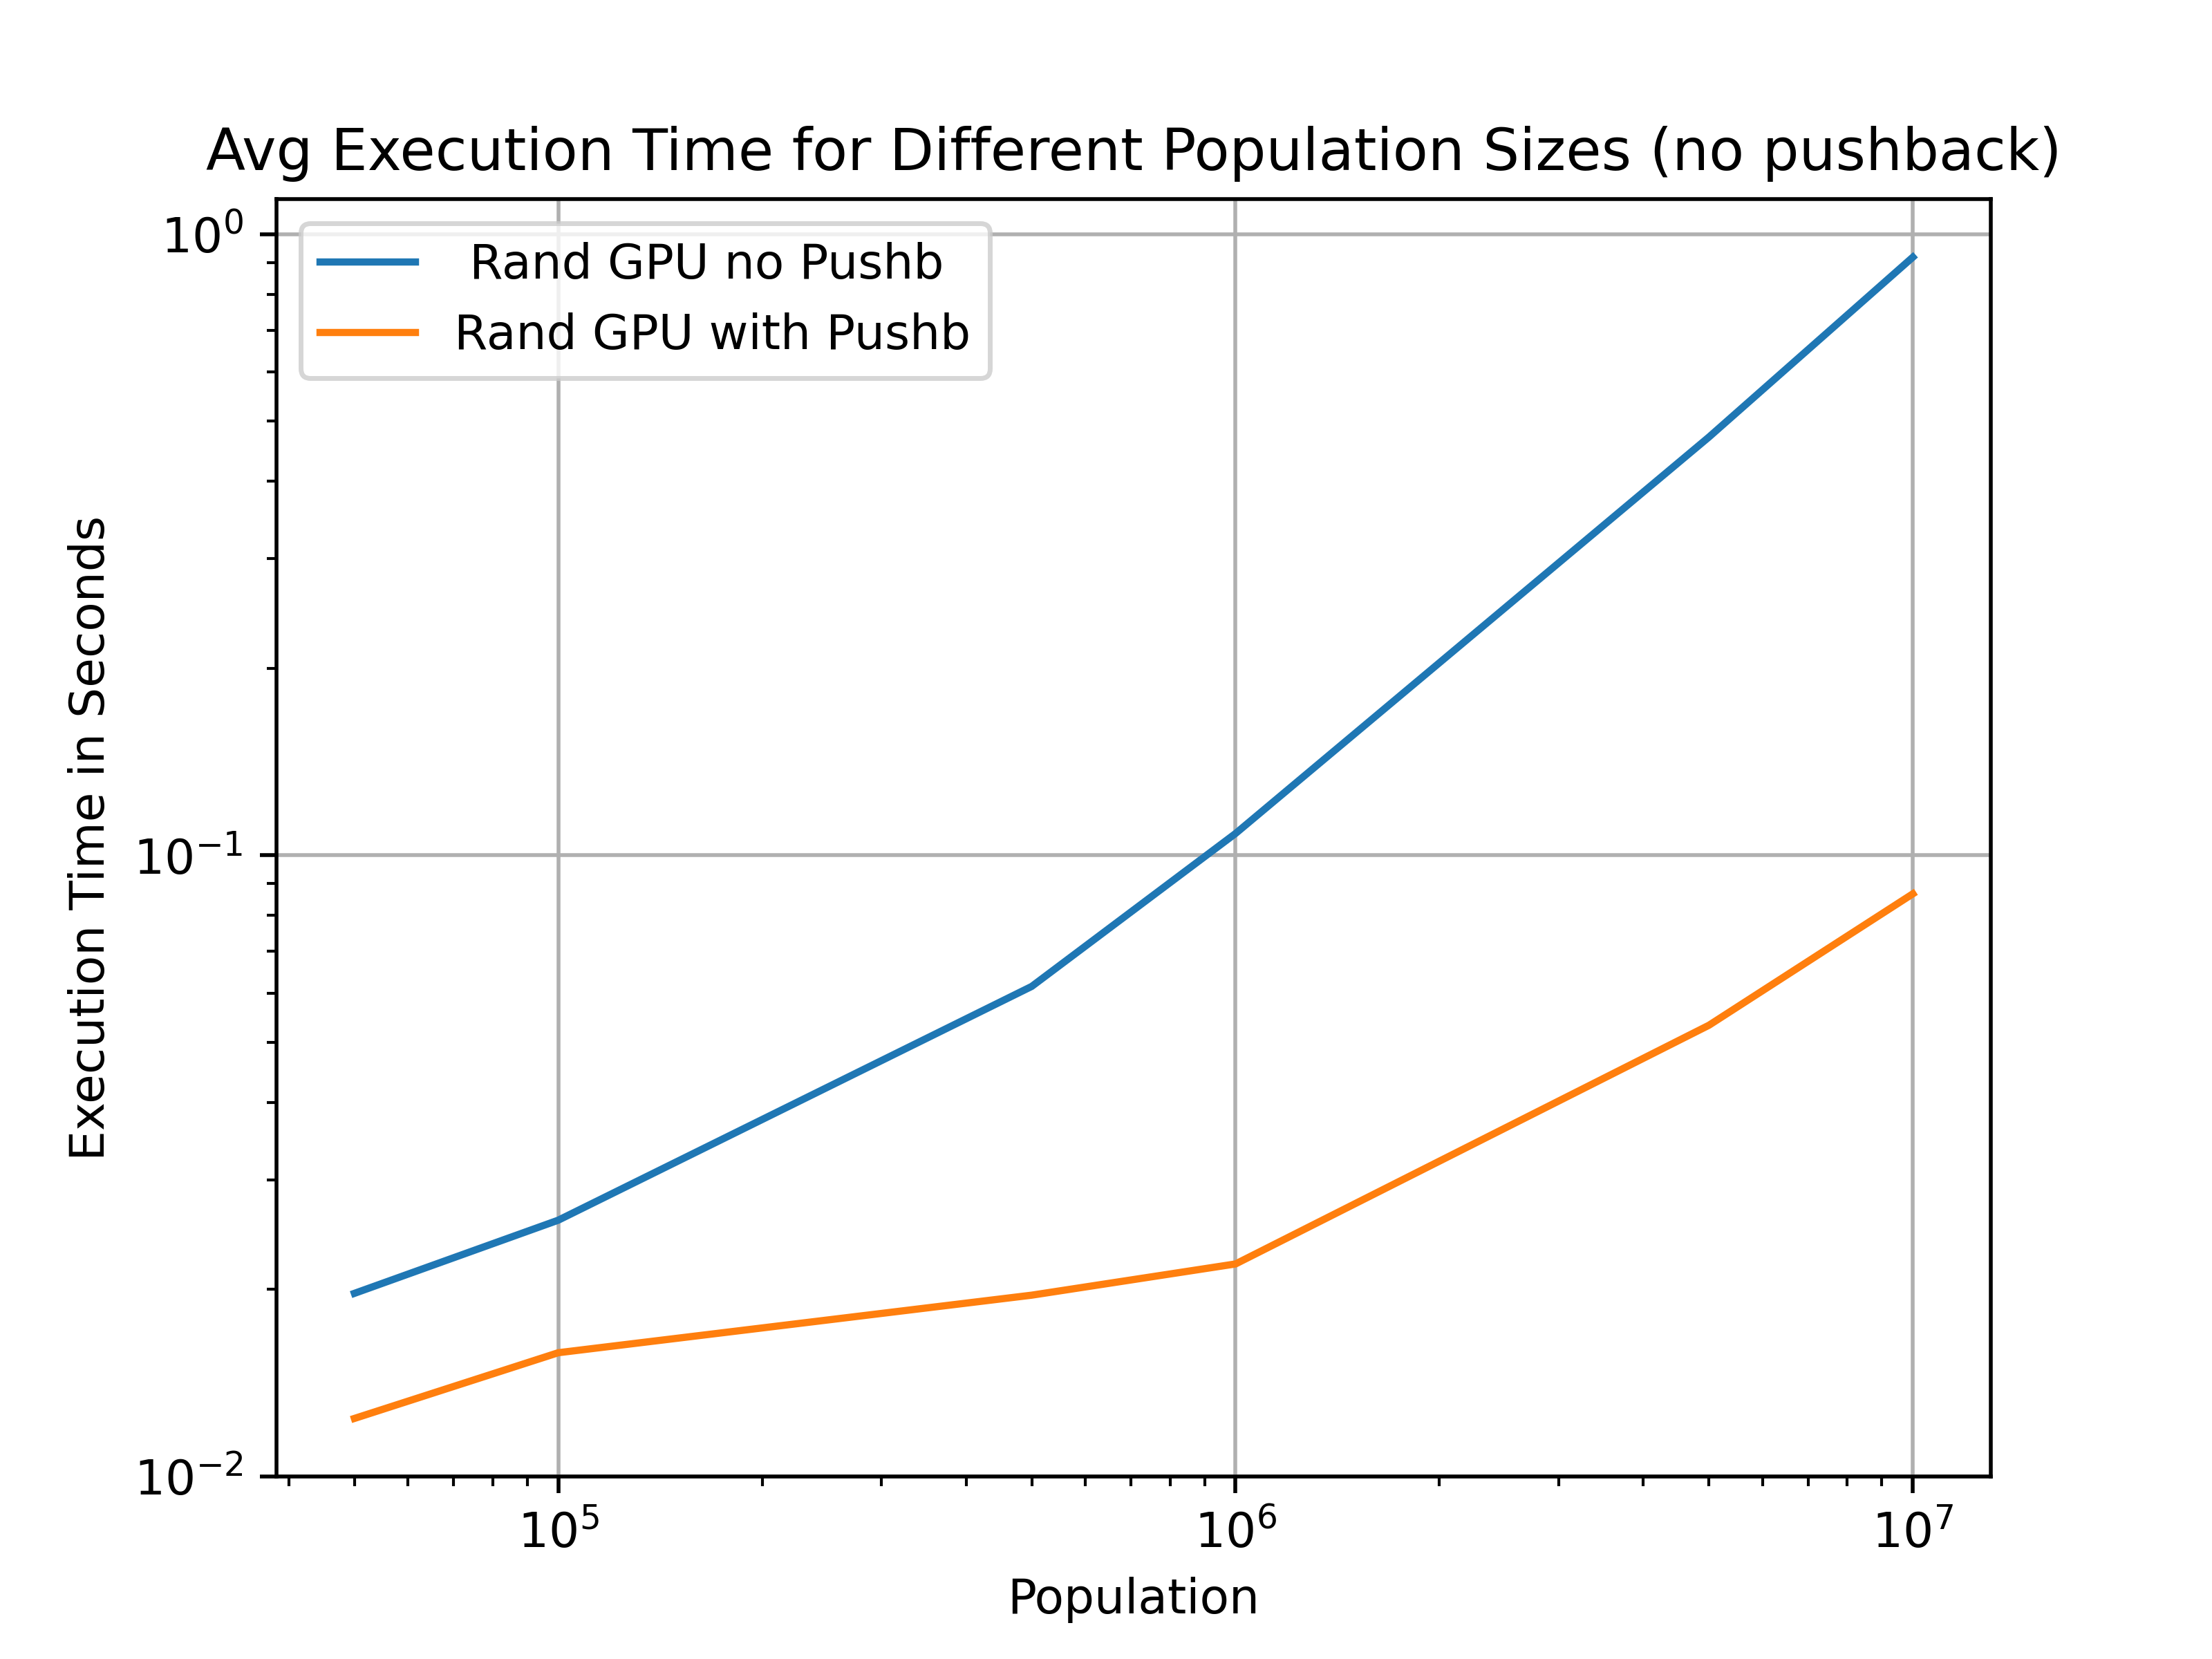
\includegraphics[width=12cm]{../Population_no_push.png}
    \caption{Execution times with pushback for different ppopulation sizes(with and withou pushback).}
    \label{fig:population_no_push}
\end{figure}

Another aspect that influences performance is the number of contacts each person has on each day. In the following plot the random number generator on the GPU is used to show the impact of the number of contacts of each person each day. To have a better understanding of the scaling the days were varied but pushback was disabled to get the full picture of the simulated days. 
\begin{figure}[H]
  \centering
  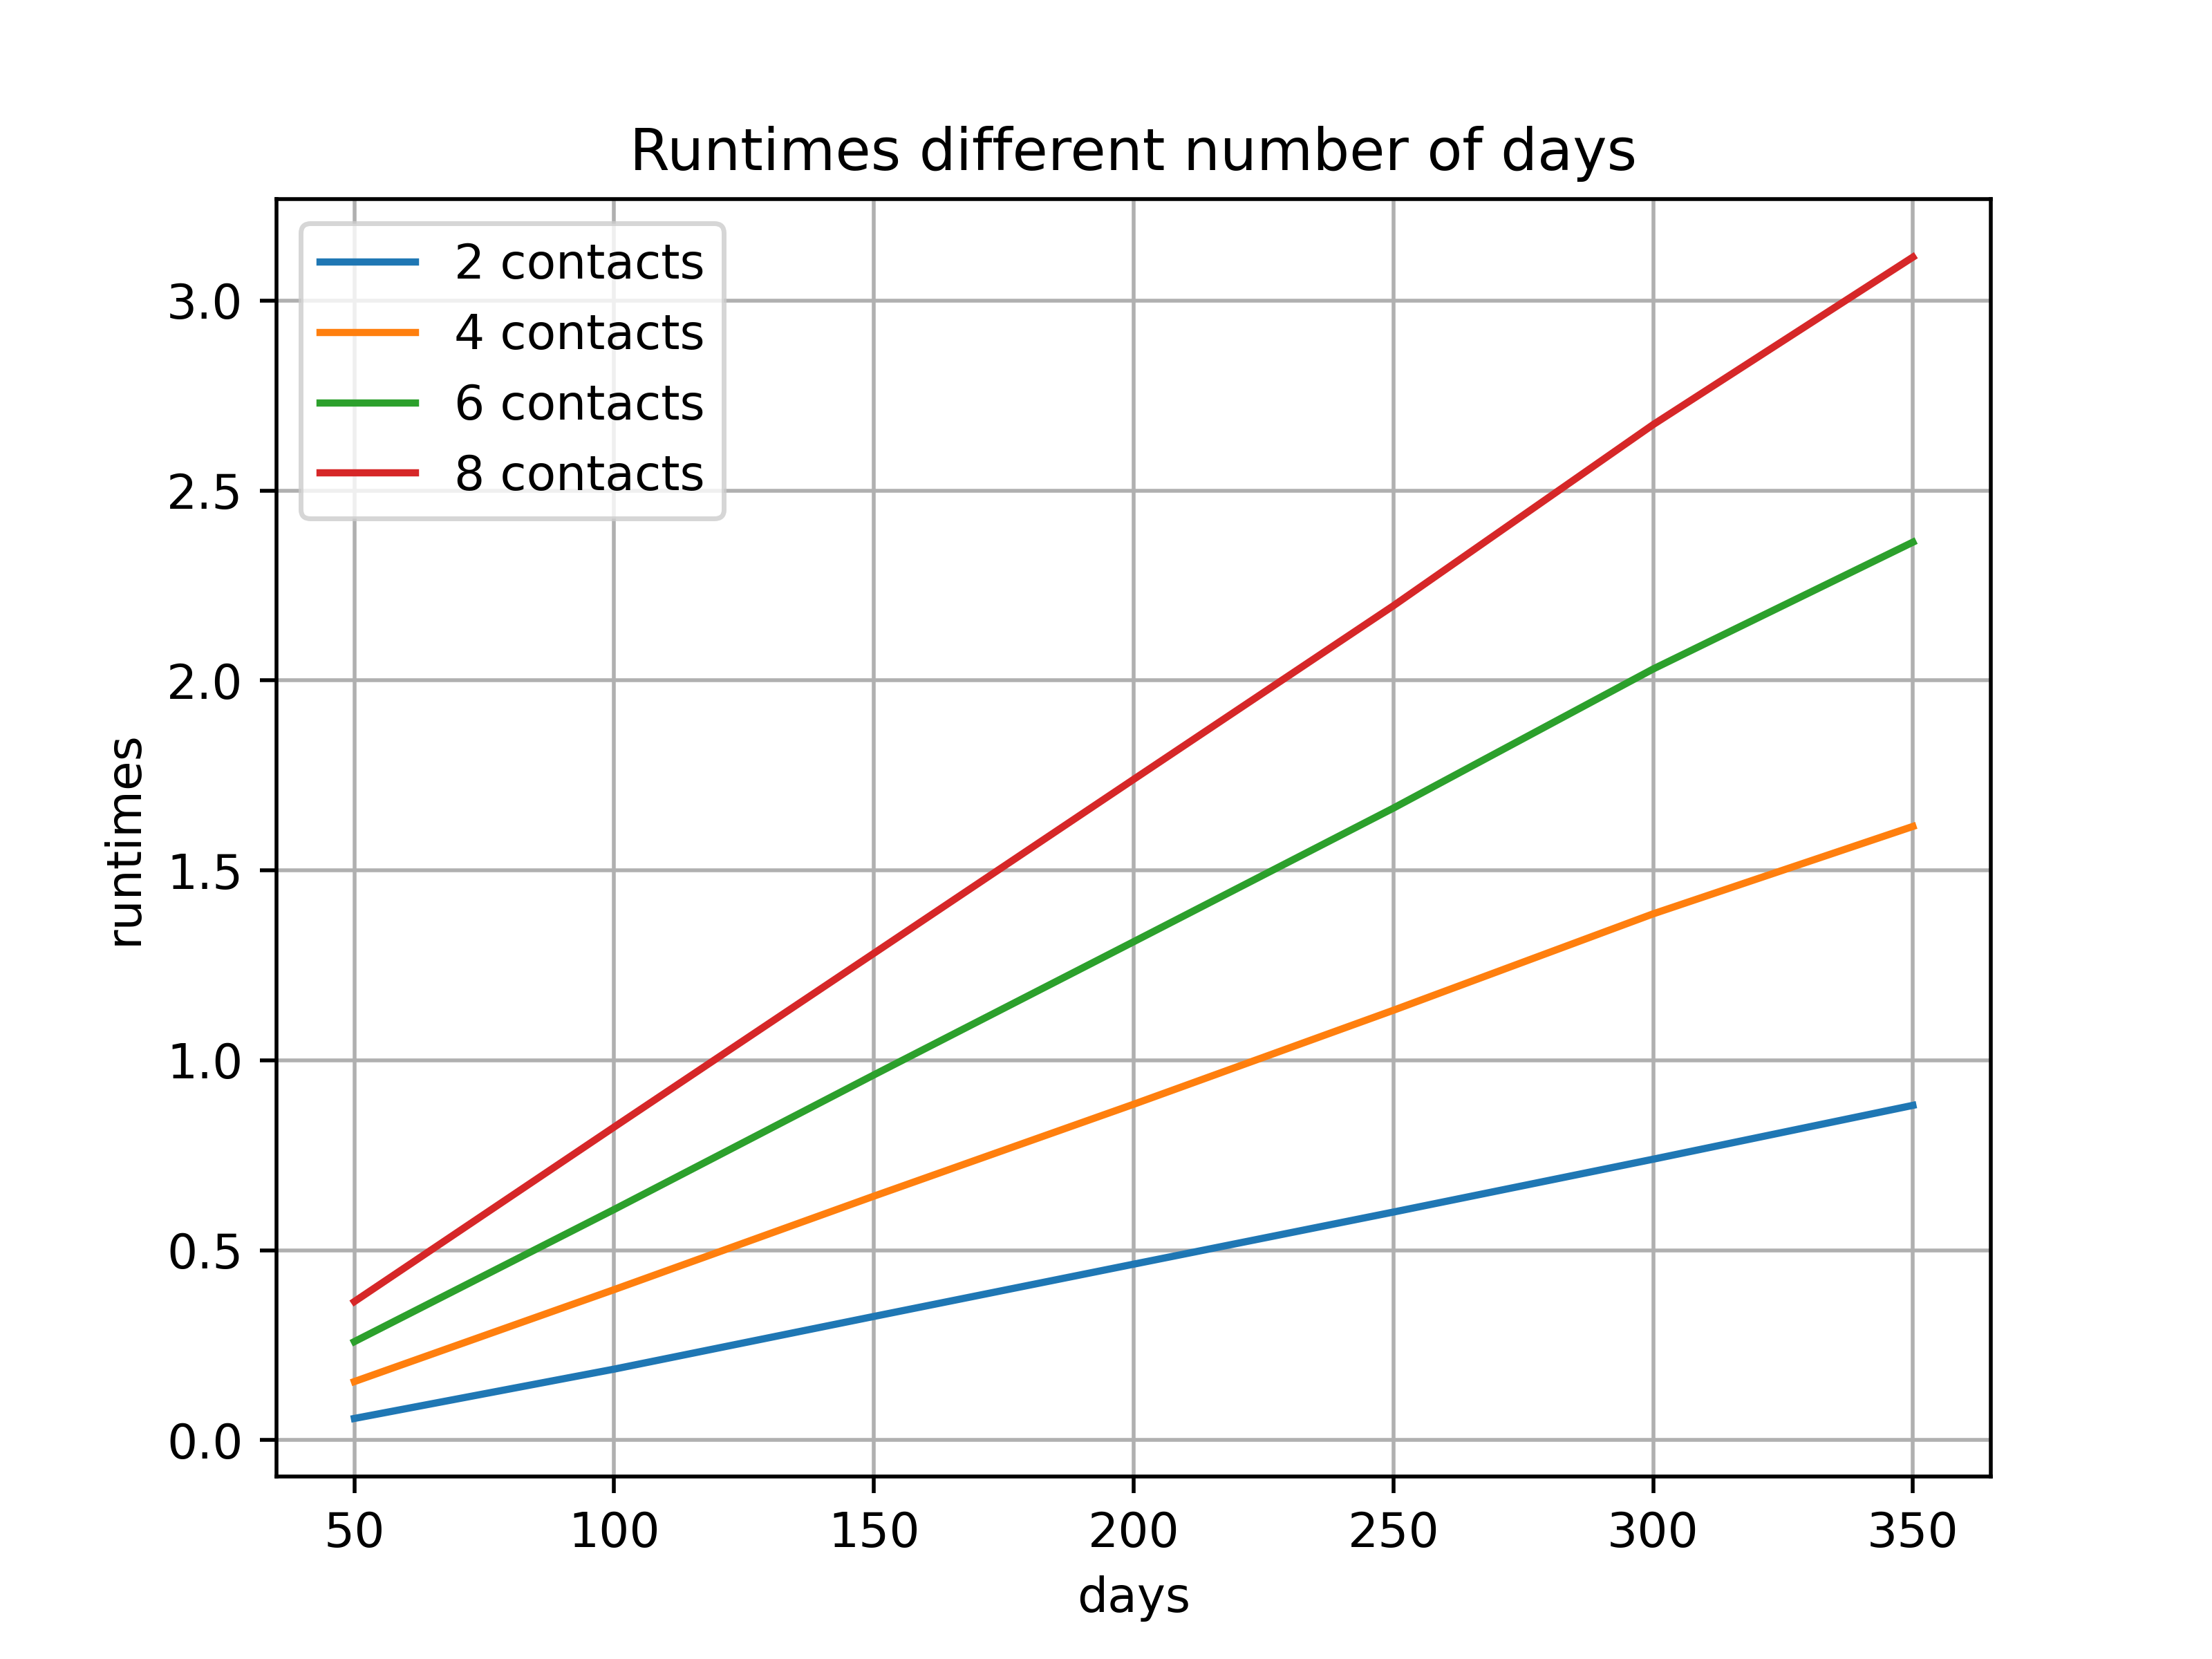
\includegraphics[width=12cm]{../contacts.png}
  \caption{Execution times for different number of days for  different number of contacts.}
  \label{fig:contacts}
\end{figure}
To get  an idea of the overall parameters that have the most impact on the runtime of the simulation the following parameters seem to be the most important: 
\begin{itemize}
  \item \textbf{Population Size: } This has an immediat impact on the performance in every scenario, because each cuda kernel loops over the whole population.
  \item \textbf{Contacts per Day: } This parameetr is responsible for the size of the loop inside the population loop in the pass on  fakenews kernel. The impact grows as more people become believers.
  \item \textbf{Days Simulated: } This is responsible for the length of the outer most loop in the simulation function, but is mostly not fully executed due to the pushback and its effect.
\end{itemize}
So a performance model for the worst case would be 
\begin{align}
  O(Population \cdot contacts \cdot days)
\end{align}
This would be most accurate when there is no pushback and most of the people are already fakenews believers. In a normal execution with the pushback parameters this limit will probably never be reached. But it gives a good idea of the worst case and the impacts the variables have on the performance of the simulation. The most influence definitely has the population size in a normal execution.
\end{document}